\documentclass{beamer}
\usepackage{graphicx}
\usepackage{xcolor}
\usepackage{tikz}

\usepackage{colortbl}     % 支持 \rowcolor
\usepackage[table]{xcolor}  % 增强颜色支持，特别是灰色背景
\usepackage{array}        % 增强表格功能（对齐方式等）
\usepackage{booktabs



% 自定义颜色
\definecolor{purpleblue}{RGB}{80, 80, 180}
\definecolor{lightgray}{RGB}{230, 230, 230}
\definecolor{novelPurple}{RGB}{98, 54, 255} 
\definecolor{darkgray}{RGB}{50, 50, 50}

% 主题设置
\usetheme{Madrid}  
\usecolortheme{dolphin} 

% 设置字体（移除 fontspec，确保 pdfLaTeX 兼容）
\setbeamerfont{title}{size=\Large,series=\bfseries}
\setbeamerfont{frametitle}{size=\LARGE,series=\bfseries}
\setbeamercolor{frametitle}{fg=white, bg=novelPurple}
\setbeamercolor{title}{fg=white, bg=purpleblue}

% 封面信息
\title[SAT Unit 3.3 ]{\textbf{SAT Unit 3.3\\ Statistics: One Variable Data}}
\author{\textbf{Jack Zeng}}
\institute{\textcolor{white}{\textbf{Novel Prep}}}
\date{\today} 

\begin{document}

% --- Title Slide ---
\begin{frame}
    \titlepage
    \vfill
    \begin{flushright}
        \textcolor{purpleblue}{\Huge \textbf{Novel Prep}}
    \end{flushright}
\end{frame}




\begin{frame}
    \begin{tikzpicture}[remember picture, overlay]
        % 设置浅色渐变背景
        \shade[top color=softPurple, bottom color=softGray] 
            (current page.north west) rectangle (current page.south east);
        
        % 添加高斯模糊光晕
        \fill[white, opacity=0.3] (current page.center) circle (4cm);
        
        % 主标题
        \node[align=center] at (current page.center) {
            {\Huge\bfseries\textcolor{purpleblue}{Novel Prep}} \\[0.5cm]
            {\Large\itshape\textcolor{lightText}{Excellence in SAT Prep}}
        };

        % 添加柔和光点（点缀）
        \foreach \x in {1,2,3,4,5} {
            \fill[purpleblue, opacity=0.2] (rand*10-5, rand*7-3.5) circle (0.1+\x*0.05);
        }

        ;
    \end{tikzpicture}
\end{frame}


\begin{frame}{Overview}
    \tableofcontents
\end{frame}

\begin{frame}
\section{ Mean, Median, and Mode}
    \begin{tikzpicture}[remember picture, overlay]
        % 设置浅色渐变背景
        \shade[top color=softPurple, bottom color=softGray] 
            (current page.north west) rectangle (current page.south east);
        
        % 添加高斯模糊光晕
        \fill[white, opacity=0.3] (current page.center) circle (4cm);
        
        % 主标题
        \node[align=center] at (current page.center) {
            {\LARGE\bfseries\textcolor{purpleblue}{ Mean, Median, and Mode}} \\[0.5cm]
            {\Large\itshape\textcolor{lightText}{Excellence in SAT Prep}}
        };

        % 添加柔和光点（点缀）
        \foreach \x in {1,2,3,4,5} {
            \fill[purpleblue, opacity=0.2] (rand*10-5, rand*7-3.5) circle (0.1+\x*0.05);
        }

        ;
    \end{tikzpicture}
\end{frame}



\begin{frame}{Understanding Mean, Median, and Mode}
\small

\textbf{Mean (Average):}  
\[
\text{Mean} = \frac{x_1 + x_2 + \cdots + x_n}{n}
\]
\begin{itemize}
    \item \textbf{Effect of Outliers:} Extremely sensitive to outliers.
    \item \textbf{Interpretation:} Represents a balance point of the data.
    \item If one value increases by $k$, the mean increases by $\frac{k}{n}$.
\end{itemize}

\vspace{0.3cm}
\textbf{Median (Middle Value):}
\begin{itemize}
    \item The value separating the higher half from the lower half.
    \item \textbf{Robustness:} Resistant to outliers; a better measure of central tendency for skewed data.
    \item A single extreme value has no effect unless it shifts the order.
\end{itemize}

\end{frame}

\begin{frame}{More on Mean and Median with Data Behavior}
\small

\textbf{When is Median Preferred over Mean?}
\begin{itemize}
    \item Skewed data (e.g., income distribution).
    \item Presence of outliers or extreme values.
\end{itemize}

\vspace{0.3cm}
\textbf{Examples of Change Impact:}
\begin{itemize}
    \item Add 1000 to an income of $30,000$: Mean jumps; median may stay same.
    \item Remove a high outlier: Mean drops; median may remain unchanged.
\end{itemize}

\vspace{0.3cm}
\textbf{Mode:}
\begin{itemize}
    \item The value(s) that appear most frequently in a data set.
    \item May have none, one, or multiple modes.
    \item Useful for categorical or discrete data.
\end{itemize}

\end{frame}


\begin{frame}{\textbf{Data Set and Mean Problem}}
Data set \( A \) consists of 10 positive integers less than 60. The list shown gives 9 of the integers from data set \( A \):

\[
43,\ 45,\ 44,\ 43,\ 38,\ 39,\ 40,\ 46,\ 40
\]

The mean of these 9 integers is 42. If the mean of data set \( A \) is an integer that is greater than 42, what is the value of the largest integer from data set \( A \)?
\end{frame}


\begin{frame}{\textbf{Solution to Data Set and Mean Problem}}
Let the missing number be \( x \). The sum of the 9 known numbers is:
\[
43 + 45 + 44 + 43 + 38 + 39 + 40 + 46 + 40 = 378
\]

Mean of all 10 numbers must be an integer greater than 42. So:
\[
\frac{378 + x}{10} > 42 \Rightarrow 378 + x > 420 \Rightarrow x > 42
\]

Since the mean must also be an integer, try smallest integer value for the mean greater than 42, which is 43:
\[
\frac{378 + x}{10} = 43 \Rightarrow 378 + x = 430 \Rightarrow x = 52
\]

\textbf{Correct Answer: 52}
\end{frame}

\begin{frame}{\textbf{Effect of Adding an Outlier to a Data Set}}
Data set F consists of 55 integers between 170 and 290. Data set G consists of all the integers in data set F as well as the integer 10. 

Which of the following must be less for data set F than for data set G?

\begin{enumerate}
    \item The mean
    \item The median
\end{enumerate}

\begin{itemize}
    \item[A.] I only
    \item[B.] II only
    \item[C.] I and II
    \item[D.] Neither I nor II
\end{itemize}
\end{frame}


\begin{frame}{\textbf{Answer and Explanation}}
\begin{itemize}
    \item Adding an extreme low value (like 10) to data set F will significantly reduce the \textbf{mean} of the data set, since the mean is sensitive to outliers.
    \item However, the \textbf{median} is the middle value. Since 10 is far below the range of values in set F (170–290), it will simply be placed at the beginning and not affect the central value of the sorted list.
\end{itemize}

\textbf{Conclusion:}
\begin{itemize}
    \item Mean of F $>$ Mean of G
    \item Median remains unchanged
\end{itemize}

\textbf{Correct Answer: A. I only}
\end{frame}









\begin{frame}
\section{ Standard Deviation and Range}
    \begin{tikzpicture}[remember picture, overlay]
        % 设置浅色渐变背景
        \shade[top color=softPurple, bottom color=softGray] 
            (current page.north west) rectangle (current page.south east);
        
        % 添加高斯模糊光晕
        \fill[white, opacity=0.3] (current page.center) circle (4cm);
        
        % 主标题
        \node[align=center] at (current page.center) {
            {\LARGE\bfseries\textcolor{purpleblue}{ Standard Deviation and Range}} \\[0.5cm]
            {\Large\itshape\textcolor{lightText}{Excellence in SAT Prep}}
        };

        % 添加柔和光点（点缀）
        \foreach \x in {1,2,3,4,5} {
            \fill[purpleblue, opacity=0.2] (rand*10-5, rand*7-3.5) circle (0.1+\x*0.05);
        }

        ;
    \end{tikzpicture}
\end{frame}


\begin{frame}{Standard Deviation: Definition and Analysis}
\small

\textbf{Definition:}
\[
\sigma = \sqrt{\frac{1}{n} \sum_{i=1}^n (x_i - \mu)^2}
\]
\begin{itemize}
    \item Measures the \textbf{spread} or \textbf{dispersion} of data around the mean.
    \item A small $\sigma$ indicates data points are close to the mean.
    \item A large $\sigma$ implies data is more spread out.
\end{itemize}

\vspace{0.3cm}
\textbf{How It Changes:}
\begin{itemize}
    \item Adding a constant to all values: $\sigma$ stays the same.
    \item Multiplying all values by a constant $k$: $\sigma$ becomes $|k|\sigma$.
    \item Introducing an outlier: $\sigma$ increases significantly.
\end{itemize}

\end{frame}

\begin{frame}{Range: Definition and Behavior}
\small

\textbf{Definition:}
\[
\text{Range} = \text{Maximum value} - \text{Minimum value}
\]

\vspace{0.2cm}
\textbf{Properties:}
\begin{itemize}
    \item Measures the \textbf{total spread} of a data set.
    \item Only uses the two \textbf{extreme values}; does \textbf{not} reflect the distribution of other data points.
    \item \textbf{Sensitive to outliers} — a single large or small value can drastically change the range.
\end{itemize}

\vspace{0.2cm}
\textbf{How Range is Affected:}
\begin{itemize}
    \item Adding a constant to all values: \textbf{No change} in range.
    \item Multiplying all values by a positive constant $k$: Range becomes $k \cdot \text{(original range)}$.
    \item Replacing max or min with a more extreme value increases the range.
\end{itemize}
\end{frame}


\begin{frame}{\textbf{Modified Data Set and Statistical Measures}}
A data set of 27 different numbers has a mean of 33 and a median of 33. A new data set is created by adding 7 to each number in the original data set that is greater than the median and subtracting 7 from each number in the original data set that is less than the median.

Which of the following measures does \textbf{NOT} have the same value in both the original and new data sets?

\begin{itemize}
    \item[A.] Median
    \item[B.] Mean
    \item[C.] Sum of the numbers
    \item[D.] Standard deviation
\end{itemize}
\end{frame}

\begin{frame}{\textbf{Answer and Explanation}}
\begin{itemize}
    \item The \textbf{median} stays the same, since the middle number (33) is unchanged.
    \item The \textbf{mean} unchanged.
    \item The \textbf{sum} of the values changes for the same reason the mean does — because of the increases and decreases.
    \item The \textbf{standard deviation} increases, since numbers are being moved further from the center (more spread).
\end{itemize}

The only measure that does \textbf{not} stay the same is the:
\[
\textbf{Correct Answer: D. Standard Deviation}
\]
\end{frame}





\begin{frame}
\section{Frequency Table, Dot Plot, Bar Graphs, and Histogram}
    \begin{tikzpicture}[remember picture, overlay]
        % 设置浅色渐变背景
        \shade[top color=softPurple, bottom color=softGray] 
            (current page.north west) rectangle (current page.south east);
        
        % 添加高斯模糊光晕
        \fill[white, opacity=0.3] (current page.center) circle (4cm);
        
        % 主标题
        \node[align=center] at (current page.center) {
            {\large\bfseries\textcolor{purpleblue}{ Frequency Table, Dot Plot, Bar Graphs, and Histogram}} \\[0.5cm]
            {\Large\itshape\textcolor{lightText}{Excellence in SAT Prep}}
        };

        % 添加柔和光点（点缀）
        \foreach \x in {1,2,3,4,5} {
            \fill[purpleblue, opacity=0.2] (rand*10-5, rand*7-3.5) circle (0.1+\x*0.05);
        }

        ;
    \end{tikzpicture}
\end{frame}


\begin{frame}{Dot Plot}


A \textbf{dot plot} is a simple way to display numerical data using dots. Each dot represents one occurrence of a data value, and the dots are stacked vertically above a number line corresponding to the data values.


    \begin{center}
    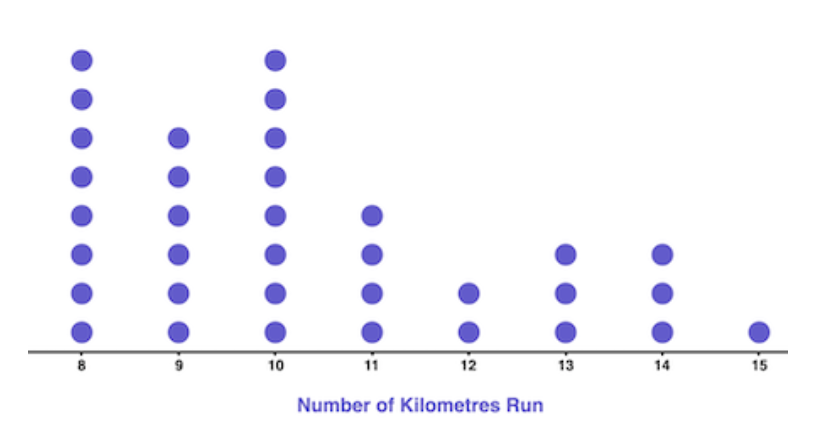
\includegraphics[width=0.8\linewidth]{E28.png}
    \end{center}
\end{frame}

\begin{frame}{Histogram}

A \textbf{Histogram} is a type of bar graph that represents the \textbf{frequency distribution} of a dataset. It displays data in intervals (also called bins), where the height of each bar corresponds to the frequency of data within that interval. Unlike bar charts, there are \textbf{no gaps} between the bars in a histogram.


    \begin{center}
    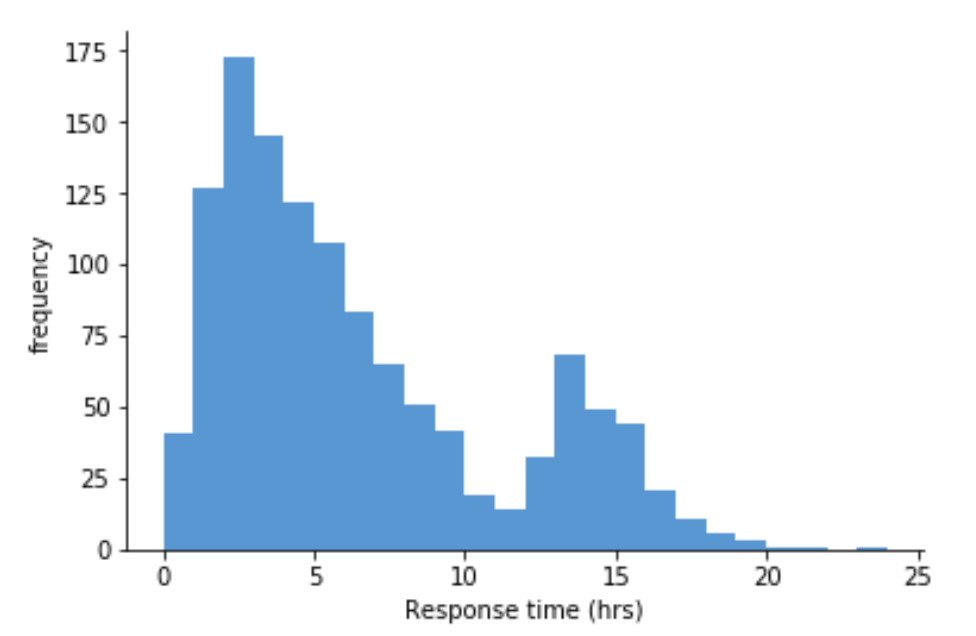
\includegraphics[width=0.7\linewidth]{E29.png}
    \end{center}
\end{frame}



\begin{frame}{Box Plot}
\small


A \textbf{box plot}, also known as a box-and-whisker plot, graphically represents the \textbf{five-number summary}:
\[
\text{Minimum}, \quad Q_1 \ (\text{First Quartile}), \quad \text{Median}, \quad Q_3 \ (\text{Third Quartile}), \quad \text{Maximum}
\]

    \begin{center}
    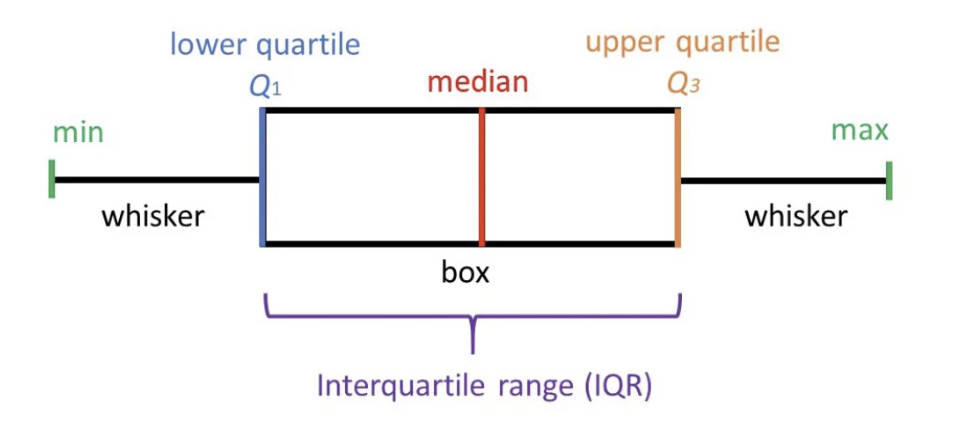
\includegraphics[width=0.8\linewidth]{E30.png}
    \end{center}
\end{frame}
    
\end{frame}
    
\end{frame}

\begin{frame}{Contingency Table (Two-Way Table)}
\small
        A \textbf{Contingency Table} or \textbf{Two-Way Table} summarizes the frequency of occurrences for two categorical variables. It helps analyze the relationship between these variables by organizing data into rows and columns.

        \vspace{5mm}
        The table below shows the relationship between students' \textbf{Gender} and their \textbf{Preference for Study Subject}.

\begin{center}
\begin{tabular}{|l|c|c|c|c|}
\hline
\rowcolor[HTML]{EFEFEF}
\textbf{Gender} & \textbf{Math} & \textbf{Science} & \textbf{History} & \textbf{Total} \\
\hline
\textbf{Male}   & 20 & 25 & 15 & 60 \\
\textbf{Female} & 30 & 20 & 40 & 90 \\
\hline
\textbf{Total}  & 50 & 45 & 55 & 150 \\
\hline
\end{tabular}
\end{center}



\end{frame}

\begin{frame}
{\textbf{Box Plot Interpretation – Mass Comparison}}
\small
The box plots summarize the masses, in kilograms, of two groups of gazelles. Based on the box plots, which of the following statements \textbf{must be true}?

\begin{itemize}
    \item[A] The mean mass of group 1 is greater than the mean mass of group 2.
    \item[B]The mean mass of group 1 is less than the mean mass of group 2.
    \item[C] The median mass of group 1 is greater than the median mass of group 2.
    \item[D] The median mass of group 1 is less than the median mass of group 2.
\end{itemize}

    \begin{center}
    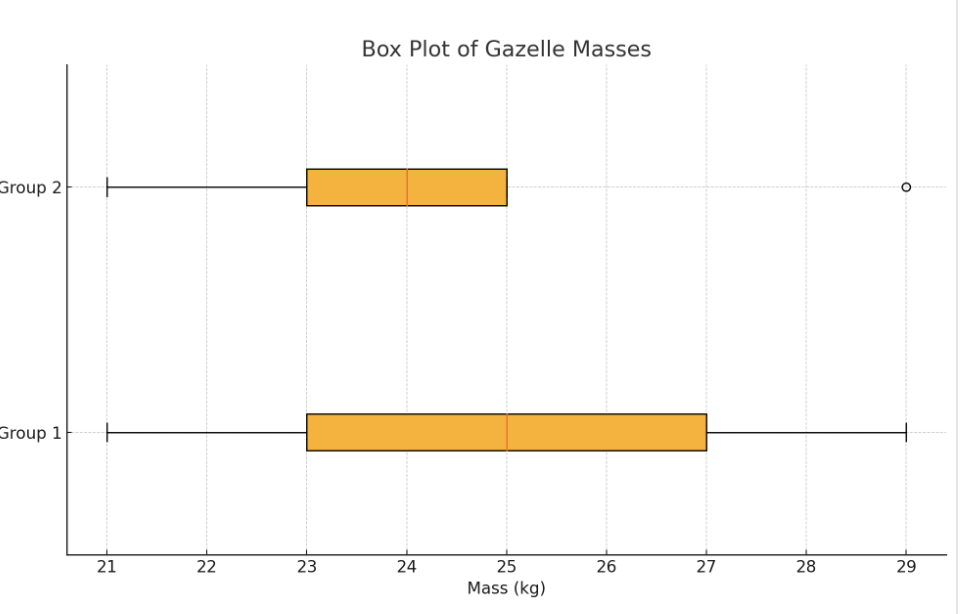
\includegraphics[width=0.55\linewidth]{E31.png}
    \end{center}
\end{frame}


\begin{frame}{\textbf{Answer and Explanation}}
\begin{itemize}
    \item The median of group 1 is clearly to the right of the median of group 2.
    \item Since median values are shown as vertical lines inside each box, it is evident that:
    \[
    \text{Median}_{\text{Group 1}} > \text{Median}_{\text{Group 2}}.
    \]
    \item Statements about the mean \textbf{cannot} be verified from a box plot alone.
\end{itemize}

\textbf{Correct Answer: C}
\end{frame}


\begin{frame}{\textbf{Dot Plot and Data Transformation }}
\footnotesize
\begin{center}
    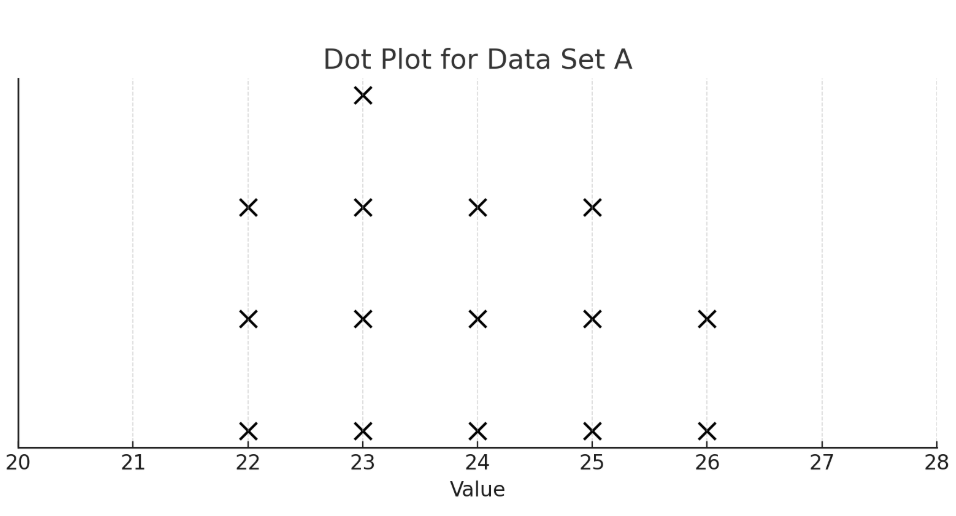
\includegraphics[width=0.40\linewidth]{E32.png}
\end{center}
The dot plot represents the 15 values in data set A. Data set B is created by adding \( 56 \) to each of the values in data set A. 

Which of the following correctly compares the medians and the ranges of data sets A and B?

\begin{itemize}
        \item [A] The median of data set B is equal to the median of data set A, and the range of data set B is equal to the range of data set A.
        \item [B] The median of data set B is equal to the median of data set A, and the range of data set B is greater than the range of data set A.
        \item [C] The median of data set B is greater than the median of data set A, and the range of data set B is equal to the range of data set A.
        \item [D] The median of data set B is greater than the median of data set A, and the range of data set B is greater than the range of data set A.
\end{itemize}
\end{frame}


\begin{frame}{\textbf{Answer and Explanation}}
\begin{itemize}
    \item Adding the same number to all values in a data set increases the median by that amount.
    \item However, the spread (range) remains unchanged because both the maximum and minimum values are increased equally.
    \item Thus:
    \begin{itemize}
        \item \textbf{Median of B} is greater than \textbf{median of A}
        \item \textbf{Range of B} is equal to \textbf{range of A}
    \end{itemize}
\end{itemize}

\textbf{Correct Answer: C}
\end{frame}







\begin{frame}{\textbf{Median Comparison – Grouped Data}}
\small
For a certain computer game, individuals receive an integer score that ranges from 2 through 10. The table below shows the frequency distribution of the scores of the 9 players in group A and the 11 players in group B.

\begin{center}
\begin{tabular}{|c|c|c|}
\hline
\textbf{Score} & \textbf{Group A} & \textbf{Group B} \\
\hline
2 & 1 & 0 \\
3 & 1 & 0 \\
4 & 2 & 0 \\
5 & 1 & 4 \\
6 & 3 & 2 \\
7 & 0 & 0 \\
8 & 0 & 2 \\
9 & 1 & 1 \\
10 & 0 & 2 \\
\hline
\textbf{Total} & 9 & 11 \\
\hline
\end{tabular}
\end{center}

\vspace{2mm}
\textbf{Question:} The median of the scores for group B is how much greater than the median of the scores for group A?
\end{frame}


\begin{frame}{\textbf{Answer – Median Comparison}}
To find the medians:

\begin{itemize}
    \item \textbf{Group A (9 players):} Median is the 5\textsuperscript{th} value.
    
    Sorted values based on frequency:
    \[
    2,\ 3,\ 4,\ 4,\ \boxed{5},\ 6,\ 6,\ 6,\ 9
    \]
    Median of Group A = \( \boxed{5} \)
    
    \item \textbf{Group B (11 players):} Median is the 6\textsuperscript{th} value.
    
    Sorted values based on frequency:
    \[
    5,\ 5,\ 5,\ 5,\ 6,\ \boxed{6},\ 8,\ 8,\ 9,\ 10,\ 10
    \]
    Median of Group B = \( \boxed{6} \)
\end{itemize}

\textbf{Final Answer:} The median of group B is \( \boxed{1} \) greater than the median of group A.
\end{frame}


\begin{frame}
    \begin{tikzpicture}[remember picture, overlay]
        % 设置浅色渐变背景
        \shade[top color=softPurple, bottom color=softGray] 
            (current page.north west) rectangle (current page.south east);
        
        % 添加高斯模糊光晕
        \fill[white, opacity=0.3] (current page.center) circle (4cm);
        
        % 主标题
        \node[align=center] at (current page.center) {
            {\Huge\bfseries\textcolor{purpleblue}{Practices}} \\[0.5cm]
            {\Large\itshape\textcolor{lightText}{Excellence in SAT Prep}}
        };

        % 添加柔和光点（点缀）
        \foreach \x in {1,2,3,4,5} {
            \fill[purpleblue, opacity=0.2] (rand*10-5, rand*7-3.5) circle (0.1+\x*0.05);
        }

        ;
    \end{tikzpicture}
\end{frame}


\begin{frame}{Question}
Data set P: 41, 43, 45, 45, 47, 47, 51, 51, 55 \\
Data set Q: 33, 33, 36, 36, 38, 38, 40, 40, 40 \\
\\
The data values for data sets P and Q are shown. The median of data set P is how much greater than the median of data set Q?
\end{frame}


\begin{frame}{Answer}
\textbf{Step 1. Find the median of data set P:} \\
Data set P (ordered): 41, 43, 45, 45, 47, 47, 51, 51, 55 \\
Median: 47 \\
\\
\textbf{Step 2. Find the median of data set Q:} \\
Data set Q (ordered): 33, 33, 36, 36, 38, 38, 40, 40, 40 \\
Median: 38 \\
\\
\textbf{Step 3. Difference:} \\
47 - 38 = 9 \\
\\
\textbf{Answer:} The median of data set P is 9 greater than the median of data set Q.
\end{frame}

\begin{frame}{Question}
The frequency table summarizes the prices of 30 items in a shopping cart.

\begin{center}
\begin{tabular}{|c|c|}
\hline
\textbf{Price (dollars)} & \textbf{Frequency} \\
\hline
25 & 8 \\
40 & 2 \\
45 & 4 \\
55 & 10 \\
70 & 6 \\
\hline
\end{tabular}
\end{center}

If an item with a price of 25 dollars is removed from the shopping cart, what will be the effect on the mean and median price of the items in the shopping cart?

\begin{enumerate}[A.]
    \item The mean and median will both decrease.
    \item The mean and median will both increase.
    \item The mean will decrease, and the median will remain the same.
    \item The mean will increase, and the median will remain the same.
\end{enumerate}
\end{frame}


\begin{frame}{Answer}
\textbf{Step 1. Mean Analysis:} \\
Removing a low-priced item (25) from the dataset will increase the overall mean, because the total sum decreases by less than proportionally compared to the decrease in count.

\textbf{Step 2. Median Analysis:} \\
Since there are 30 items initially, the median is the average of the 15th and 16th values when ordered. After removing one item priced at 25 (the lowest), there are now 29 items. The new median is the 15th value, which remains at 55.

\textbf{Conclusion:} \\
The mean will increase, and the median will remain the same.

\textbf{Answer:} D.
\end{frame}


\begin{frame}{Question}
\scriptsize
The tables give the distribution of daily travel times between two towns for bus A and bus B over a 40-day period.

\begin{center}
\textbf{Bus A}
\begin{tabular}{|c|c|}
\hline
Travel time (minutes) & Frequency \\
\hline
44 & 5 \\
45 & 10 \\
47 & 15 \\
48 & 10 \\
\hline
\end{tabular}
\end{center}

\begin{center}
\textbf{Bus B}
\begin{tabular}{|c|c|}
\hline
Travel time (minutes) & Frequency \\
\hline
25 & 5 \\
30 & 10 \\
35 & 15 \\
40 & 10 \\
\hline
\end{tabular}
\end{center}

Which statement correctly compares the standard deviations of travel times for bus A and bus B?

\begin{enumerate}[A.]
    \item The standard deviation of travel times for bus A is less than the standard deviation of travel times for bus B.
    \item The standard deviation of travel times for bus B is less than the standard deviation of travel times for bus A.
    \item The standard deviation of travel times for bus A is equal to the standard deviation of travel times for bus B.
    \item There is not enough information to compare these standard deviations.
\end{enumerate}
\end{frame}

\begin{frame}{Answer}
\textbf{Step 1. Check the range of values:}
\begin{itemize}
    \item Bus A: 44 to 48 (Range = 4)
    \item Bus B: 25 to 40 (Range = 15)
\end{itemize}

\textbf{Step 2. Analyze spread:}
\begin{itemize}
    \item Bus A values are clustered closer together.
    \item Bus B values are more spread out.
\end{itemize}

\textbf{Conclusion:}
Bus B has a larger standard deviation than Bus A.

\textbf{Answer:} A.
\end{frame}


\begin{frame}{Question}
\tiny
\textbf{Data set A}
\begin{center}
\begin{tabular}{|c|c|}
\hline
\textbf{Value} & \textbf{Frequency} \\
\hline
30 & 11 \\
50 & 11 \\
70 & 11 \\
\hline
\end{tabular}
\end{center}

The frequency table shown represents data set A. Which of the following frequency tables represents a data set that has a mean greater than the mean of data set A?

\begin{enumerate}[A.]
    \item 
    \begin{tabular}{|c|c|}
    \hline
    \textbf{Value} & \textbf{Frequency} \\
    \hline
    30 & 12 \\
    50 & 12 \\
    70 & 12 \\
    \hline
    \end{tabular}

    \item 
    \begin{tabular}{|c|c|}
    \hline
    \textbf{Value} & \textbf{Frequency} \\
    \hline
    30 & 9 \\
    50 & 10 \\
    70 & 11 \\
    \hline
    \end{tabular}

    \item 
    \begin{tabular}{|c|c|}
    \hline
    \textbf{Value} & \textbf{Frequency} \\
    \hline
    30 & 12 \\
    50 & 11 \\
    70 & 10 \\
    \hline
    \end{tabular}

    \item 
    \begin{tabular}{|c|c|}
    \hline
    \textbf{Value} & \textbf{Frequency} \\
    \hline
    30 & 13 \\
    50 & 11 \\
    70 & 13 \\
    \hline
    \end{tabular}
\end{enumerate}
\end{frame}

\begin{frame}{Answer}
\textbf{Step 1. Mean of data set A:}
\[
\text{Mean} = \frac{(30 \cdot 11) + (50 \cdot 11) + (70 \cdot 11)}{33}
= \frac{330 + 550 + 770}{33}
= \frac{1650}{33}
= 50.
\]

\textbf{Step 2. Compare each option:}
\begin{itemize}
    \item A: All frequencies are equal, mean = 50 (same as set A).
    \item B: More weight on 70 and less on 30, so mean > 50.
    \item C: More weight on 30, mean < 50.
    \item D: Equal frequencies on 30 and 70 but same as set A on 50; mean = 50.
\end{itemize}

\textbf{Answer:} B.
\end{frame}

\begin{frame}{Question}
\scriptsize

\textbf{Data set A and Data set B}
\begin{center}
\begin{tabular}{|c|c|@{\hspace{1cm}}|c|c|}
\hline
\multicolumn{2}{|c|}{\textbf{Data set A}} & \multicolumn{2}{c|}{\textbf{Data set B}} \\
\hline
\textbf{Value} & \textbf{Frequency} & \textbf{Value} & \textbf{Frequency} \\
\hline
10 & 2 & 13 & 2 \\
11 & 3 & 14 & 3 \\
12 & 7 & 15 & 7 \\
13 & 3 & 16 & 3 \\
14 & 9 & 17 & 9 \\
15 & 5 & 18 & 5 \\
\hline
\end{tabular}
\end{center}



The tables show the frequencies of the values for data sets A and B. Which of the following statements best compares the means and the standard deviations of data sets A and B?

\begin{enumerate}[A.]
    \item The mean of data set B is equal to the mean of data set A, and the standard deviation of data set B is equal to the standard deviation of data set A.
    \item The mean of data set B is equal to the mean of data set A, and the standard deviation of data set B is greater than the standard deviation of data set A.
    \item The mean of data set B is greater than the mean of data set A, and the standard deviation of data set B is equal to the standard deviation of data set A.
    \item The mean of data set B is greater than the mean of data set A, and the standard deviation of data set B is greater than the standard deviation of data set A.
\end{enumerate}
\end{frame}





\begin{frame}{Answer}
\textbf{Step 1. Compare the means:}
\begin{itemize}
    \item Data set B is a translation of data set A by adding 3 to each value.
    \item Therefore, the mean of data set B is 3 more than the mean of data set A.
\end{itemize}

\textbf{Step 2. Compare the standard deviations:}
\begin{itemize}
    \item Adding a constant shifts all data points equally, so standard deviation does not change.
    \item Therefore, the standard deviation of data set B is equal to that of data set A.
\end{itemize}

\textbf{Conclusion:}
\begin{itemize}
    \item The mean of data set B is greater than the mean of data set A.
    \item The standard deviations of data sets A and B are equal.
\end{itemize}

\textbf{Answer:} C.
\end{frame}















\begin{frame}{}
    \begin{tikzpicture}[remember picture, overlay]
        % 背景渐变色：蓝紫到白
        \shade[top color=novelPurple!40, bottom color=white]
            (current page.north west) rectangle (current page.south east);

        % 中心柔光
        \fill[white, opacity=0.15] (current page.center) circle (5cm);

        % 柔和光点点缀
        \foreach \x in {1,2,3,4,5} {
            \fill[novelPurple, opacity=0.12] (rand*10-5, rand*7-3.5) circle (0.1+\x*0.05);
        }
    \end{tikzpicture}

    \centering
    \vspace{5em}

    {\Huge \textbf{\textcolor{novelPurple}{Thank You!}}} \\[1em]
    {\large \textcolor{gray}{We appreciate your time and focus.}} \\[3em]

    {\LARGE \textbf{\textcolor{novelPurple}{\textsf{Novel Prep}}}}

    \vfill
\end{frame}




\end{document}